\documentclass{article}
\usepackage[T1]{fontenc}
\usepackage{lmodern}
\usepackage{graphicx}
\usepackage{amsmath,amssymb}
\usepackage[a4paper,margin=2cm]{geometry}
\usepackage[absolute,overlay]{textpos}
\setlength{\TPHorizModule}{1mm}
\setlength{\TPVertModule}{1mm}
\usepackage[indonesian]{babel}
\usepackage{hyperref}
\setlength{\emergencystretch}{2em}
% unit: Halaman 54

\begin{document}

% === Halaman 54 (python/native) ===

Contoh substitusi di dalam block cipher DES:

• Misalkan 6-bit masukan adalah 110100

 Substitusi 6-bit masukan dengan menggunakan tabel substitusi (S-Box). 

Caranya: Nomor baris tabel (bit ke-1 dan bit ke-6) = 10 (baris 2)

                  Nomor kolom tabel (bit ke-2, 3, 4, dan 5) = 1010 (kolom 10) 


 Jadi, substitusi untuk 110100 adalah entry pada baris 2 dan kolom 10, yaitu 

entri bernillai 4 atau 0100 dalam biner.

54

0

1

2

3

0         1           2          3         4         5         6         7         8        9        10      11        12    13       14       15   

4

% deskripsi: gambar native xref 219
\noindent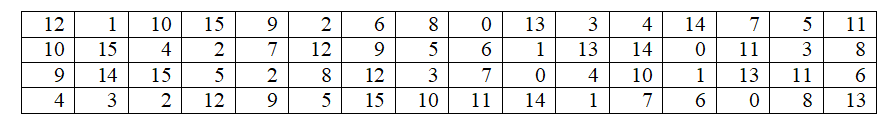
\includegraphics[width=0.85\textwidth]{../../images/python/page_054_img_01.png}

\end{document}
